\documentclass[11pt]{article} % For LaTeX2e
\usepackage[utf8]{inputenc}
\usepackage{amsmath, amsfonts, amsthm, amssymb, algorithm, graphicx}
\usepackage{mathtools}
\usepackage{enumitem}
\usepackage{pdfpages}
\usepackage[noend]{algpseudocode}
\usepackage{fancyhdr, lastpage}
\usepackage[vmargin=1.20in,hmargin=1.25in,centering,letterpaper]{geometry}
\setlength{\headsep}{.10in}
\setlength{\headheight}{15pt}
 
% Macros
\DeclareMathOperator{\BigOm}{\mathcal{O}}
\newcommand{\BigOh}[1]{\BigOm\left({#1}\right)}
\DeclareMathOperator{\BigTm}{\Theta}
\newcommand{\BigTheta}[1]{\BigTm\left({#1}\right)}
\DeclareMathOperator{\BigWm}{\Omega}
\newcommand{\BigOmega}[1]{\BigWm\left({#1}\right)}
\DeclareMathOperator{\LittleOm}{\mathrm{o}}
\newcommand{\LittleOh}[1]{\LittleOm\left({#1}\right)}
\DeclareMathOperator{\LittleWm}{\omega}
\newcommand{\LittleOmega}[1]{\LittleWm\left({#1}\right)}

\newcommand{\calW}{\mathcal{W}}

\newcommand{\calY}{\mathcal{Y}}
\newcommand{\calS}{\mathcal{S}}
\newcommand{\calD}{\mathcal{D}}
\newcommand{\calN}{\mathcal{N}}

\newcommand{\calU}{\mathcal{U}}
\newcommand{\Alt}{\mathrm{Alt}}
\newcommand{\kl}{\mathrm{kl}}
\newcommand{\calA}{\mathcal{A}}
\newcommand{\calP}{\mathcal{P}}



\newcommand{\calH}{\mathcal{H}}

\newcommand{\ArgTop}{\mathrm{ArgTop}}
\newcommand{\Top}{\mathrm{Top}}
\newcommand{\TopEps}{\mathrm{Top}^{\epsilon}}
\newcommand{\ArgTopEps}{\mathrm{ArgTop}^{\epsilon}}


\newcommand{\KL}{\mathrm{KL}}
\newcommand{\Sym}{\mathrm{Sym}}
\newcommand{\Alg}{\mathrm{Alg}}
\newcommand{\Sim}{\mathrm{Sim}}


\newcommand{\istar}{i^*}
\newcommand{\im}{\mathrm{im }}
\newcommand{\Z}{\mathbb{Z}}
\newcommand{\C}{\mathbb{C}}
\newcommand{\R}{\mathbb{R}}
\newcommand{\I}{\mathbb{I}}
\newcommand{\Exp}{\mathbb{E}}
\newcommand{\Q}{\mathbb{Q}}
\newcommand{\sign}{\mathrm{sign\ }}
\newcommand{\abs}{\mathrm{abs\ }}
\newcommand{\eps}{\varepsilon}
\newcommand{\Var}{\mathrm{Var}}
\newcommand{\Cov}{\mathrm{Cov}}
\newcommand{\zo}{\{0, 1\}}
\newcommand{\SAT}{\mathit{SAT}}
\renewcommand{\P}{\mathbf{P}}
\newcommand{\NP}{\mathbf{NP}}
\newcommand{\coNP}{\co{NP}}
\newcommand{\co}[1]{\mathbf{co#1}}
\renewcommand{\Pr}{\mathbb{P}}
{
 \theoremstyle{plain}
      \newtheorem{asm}{Assumption}
}
\theoremstyle{plain}
\newtheorem{thm}{Theorem}[section]
\newtheorem{claim}[thm]{Claim}
\newtheorem{lem}[thm]{Lemma}
\newtheorem{cor}[thm]{Corollary}


\newtheorem{prop}[thm]{Proposition}

\theoremstyle{definition}
\newtheorem{defn}{Definition}[section]
\newtheorem{conj}{Conjecture}[section]
\newtheorem{exmp}{Example}[section]
\newtheorem{exc}{Exercise}[section]


\theoremstyle{remark}
\newtheorem*{rem}{Remark}
\newtheorem*{note}{Note}
\usepackage{mathtools}
\DeclarePairedDelimiter\ceil{\lceil}{\rceil}
\DeclarePairedDelimiter\floor{\lfloor}{\rfloor}

\makeatletter
\makeatother
\renewcommand{\theequation}{\arabic{section}.\arabic{equation}}
 
\algnewcommand\algorithmicinput{\textbf{INPUT:}}
\algnewcommand\INPUT{\item[\algorithmicinput]}
\algnewcommand\algorithmicoutput{\textbf{OUTPUT:}}
\algnewcommand\OUTPUT{\item[\algorithmicoutput]}
 
% Formatting Macros
 
\pagestyle{fancy}
%\chead{\sc Problem \hmwkAssignmentNum.\hmwkProblemNum}
%\chead{}
\rhead{\em Max Simchowitz}
\cfoot{}
\lfoot{}
\rfoot{\sc Page\ \thepage\ of\ \protect\pageref{LastPage}}
\renewcommand\headrulewidth{0.4pt}
\renewcommand\footrulewidth{0.4pt}

\newcommand{\qq}[1]{{\color{magenta}{(#1)}}}
\newcommand{\rb}[1]{{\color{red}{ #1}}}
\newcommand{\bl}[1]{{\color{blue}{ #1}}}
 
%%% magic code starts
%\mathcode`*=\string"8000
%\begingroup
%\catcode`*=\active
%\xdef*{\noexpand\textup{\string*}}
%\endgroup
%%% magic code ends

\title{SISO Controller Invalidation from Open Loop Experiments}

%\author{Max Simchowitz\\
%msimchow@berkeley.edu}


\begin{document}
\section{PID control}
Consider the system
\begin{figure}[h!]
  \centering
  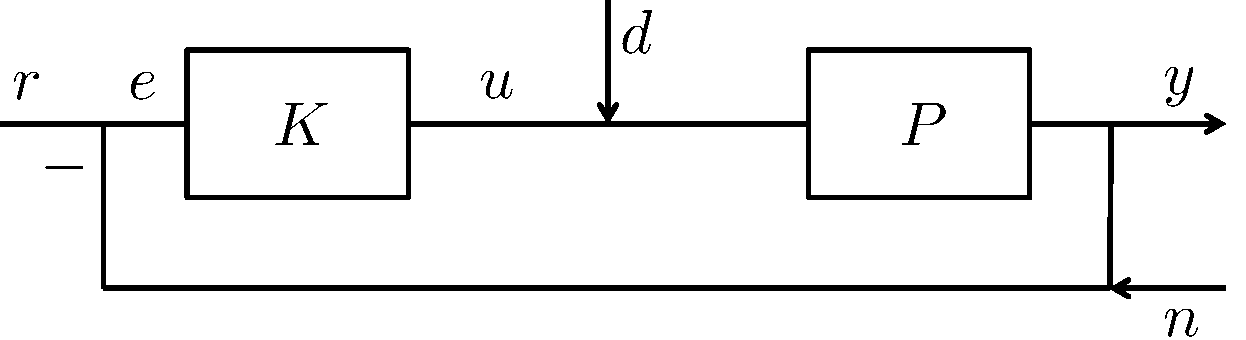
\includegraphics[width=.5\linewidth]{sys2.pdf}
\end{figure}
Our goal is to test whether a given controller $K$ can cause the plant $P$ track a known signal $r(t)$, without placing $K$ in the closed loop, over a fixed time horizon $T$. The challenge is that the plant $P$ is unkown, and lies in some class of plants $\calP$. We also assume that our plant is subject a class $\calD$ of disturbances, and noises $\calN$. We then ask if there exists a plant $P \in \calP$ such that, for any admissible disturbance $d \in \calD$ and noise $n \in \calN$, we achieve some performance objective $Q_{T,y}(r,y)$ of the reference and output. For example, $Q_{T,y} = \sum_{t=1}^T (r(t)-y(t))^{2} = \|r - y\|_{2}$. Formally, we compute
\begin{equation}\label{OPT}
\begin{aligned}
&\inf_{P \in \calP} \sup_{n \in \calN,d \in \calD} Q_{T,y}(r,y)  \\
&\text{subject to:} \quad e = r - (y+n), \quad u = Ke, y = P(u+d)
\end{aligned}
\end{equation}



For a threshold $\gamma$, we say that $K$ is \emph{invalidated} \rb{wouldn't this be more of a robust control setup? in the papers we have seen, wouldn't ``model invalidation'' be an inf inf, rather than an inf sup?} over $(\calP,\calN,\calD)$ if the optimal value of Equation~\ref{OPT} is $> \gamma$; otherwise, we say that $(\calP,\calN,\calD)$ \emph{corroborates} $K$. 
\subsection{Shrinking the set $\calP$ with open loop ID}
If $\calP$ is too unrestrictive, then the above optimization problem won't be able to invalidate a $K$ which doesn't meet the performance objective on the true plant, because there may be another plant $P' \in \calP$ for which the objective is met. Thus, we use open-loop experiments to constrain $P$. Namely, we consider the plant

\begin{figure}[h!]
  \centering
  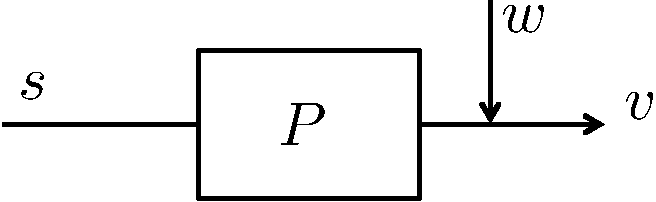
\includegraphics[width=.3\linewidth]{sys3.pdf}
\end{figure}

We then assume that take $N$ measurements of the form $v^{(j)} = Ps^{(j)} + w^{(j)}$, where $s^{(j)}$ are probe signals, and $w^{(j)}$ is stochastic noise. In the spirit of compressed sensing, we will for the moment abstract away the stochasticity of $w^{(j)}$ by assumping that the noise vectors $w = (w^{(1)},\dots,w^{(N)})$ lie in some stochastic-like set $\calW$. For example, $\calW$ can include spectral norm constraints on the matrix whose columns are formed by $w^{(j)}$ which would be celebrated by white (isotropic) noise. We will also assume that we have some prior information that $P \in \calP_0$, which we will take to control the complexity of $P$ (eg, low Hankel norm). With these constraints, we know have
\begin{equation}\label{OPT2}
\begin{aligned}
&\inf_{P \in \calP} \sup_{n \in \calN,d \in \calD} Q_{T,y}(r,y)  \\
&\text{subject to:} \quad e = r - (y+n), \quad u = Ke,\quad  y = P(u+d)\\
& P \in \calP_0, \quad w \in \calW, \quad v^{(j)} = Ps^{(j)} + w^{(j)}, j = 1,\dots,N
\end{aligned}
\end{equation}
By elimiating $e$ and $u$, we get
\begin{equation}\label{OPT3}
\begin{aligned}
&\inf_{P \in \calP} \sup_{n \in \calN,d \in \calD} Q_{T,y}(r,y)  \\
&\text{subject to:}   (I+PK)y = PKr - PKn + Pd\\
& P \in \calP_0, \quad w \in \calW, \quad v^{(j)} = Ps^{(j)} + w^{(j)}, j = 1,\dots,N
\end{aligned}
\end{equation}
\subsection{Convexity of Equation~\ref{OPT3}}
In what follows, we assume that $Q_{T,y}$ is a convex quadratic, and the sets $\calN,\calD,\calP_0,\calW$ are all convex. Thus, Equation~\ref{OPT3} suffers from only three sources of non-convexity, all in the iequality $(I+PK)y = PKr - PKn + Pd$:
\begin{enumerate}
\item  $PKy$ is bi-linear in $P$ and $y$
\item $PKn$ is bi-linear in $P$ and $n$, both of which are unkown
\item $Pd$ is bilinear in $P$ and $d$
\end{enumerate}
The latter two sources of non-convexity can be circumvented in two ways:
\begin{enumerate}
	\item Use an ``Outer Approximation'' or relaxation to the set of admissible $PKn$ and $Pd$
	\item Sample $K$ rollouts of ``typical'' noises and disturbances $\{n^{(i)},d^{(i)}\}$, and solve the optimization
	\begin{equation}\label{OPT4}
\begin{aligned}
&\inf_{P,u^{(i)},y^{(i)} \in \calP} \frac{1}{M} \sum_{i=1}^M Q(r,y^{(i)})  \\
&\text{subject to:}   (I+PK)y^{(i)} = PKr - PKn^{(i)} + Pd^{(i)}\\
& P \in \calP_0, \quad w \in \calW, \quad v^{(j)} = Ps^{(j)} + w^{(j)}, j = 1,\dots,N
\end{aligned}
\end{equation}
Note that whereas the parameter $N$ controls the number of experiments (i.e. sample complexity), $K$ controls the number of simulations (i.e. computational complexity)
\end{enumerate}
We can also rewrite the previous optimization problem in the following form:
\begin{equation}
\begin{aligned}
&\inf_{P \in \calP,y^{(i)},u^{(i)}} \frac{1}{M} \sum_{i=1}^M Q(r,y^{(i)})  \\
&\text{subject to:} \quad  y^{(i)} = Pu^{(i)}, u^{(i)} = K(r - (y^{(i)}+n^{(i)})) + d^{(i)}
\end{aligned}
\end{equation}


\subsection{}
Considering the second

\end{document}	